\begin{task}{3, Approximating nonlinear vector fields}
Our goal in this task is to explore and understand the underlying dynamics of a process. This process is characterized by two specific datasets: \textit{nonlinear\_vectorfield\_data\_x0.txt} and \textit{nonlinear\_vectorfield\_data\_x1.txt}. Each dataset comprises 2000 data points, organized into two columns, within the two-dimensional domain \([-4.5, 4.5]^2\). The dataset \textit{nonlinear\_vectorfield\_data\_x0.txt} contains the initial positions of these points, whereas \textit{nonlinear\_vectorfield\_data\_x1.txt} presents the same points after a transformation through an unknown evolution operator \(\psi\). This transformation is mathematically represented as:

\[
x^{(k)}_1 = \psi(\Delta t, x^{(k)}_0)
\]

for \( k = 1, \ldots, N \), where \( N = 2000 \) and \(\Delta t = 0.01\).
The data represented as scatter points can be seen in Figure \ref{fig:3.1}.

\begin{figure}[H]
\centering
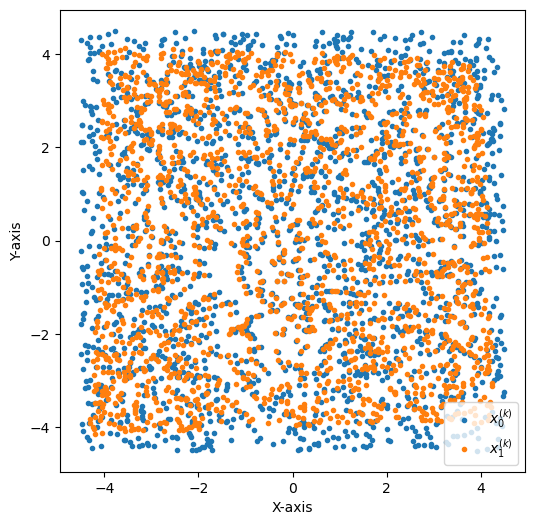
\includegraphics[width=0.5\textwidth]{images/nonlinear_vector_fields.png}
\caption{scatter points}
\label{fig:3.1}
\end{figure}

\paragraph{Part 3.1: Estimate the vector field with a linear operator}

This sub-task centered on approximating the vector field described by \(\psi\) with data from two databases. This is formulated as:

\[
\frac{d}{ds} \psi(s, x(t)) \bigg|_{s=0} \approx \hat{f}_{\text{linear}}(x(t)) = Ax(t)
\]
To determine the vector field, we computed \(\hat{v}^{(k)}\) for each data point using the formula:

\begin{equation}
\hat{v}^{(k)} = \frac{x^{(k)}_1 - x^{(k)}_0}{\Delta t}
\label{vec}
\end{equation}

Here, \(x^{(k)}_1\) and \(x^{(k)}_0\) are the known end points and initial points of the vectors, respectively. The term \(\Delta t\) represents the small time interval over which the changes in the vectors are observed.

Then we aimed to establish a relationship where the vector field 
\( \hat{v}^{(k)} \) is approximated by the product of a linear operator \( A \) and the input point \( x^{(k)}_0 \), 
expressed as \(\hat{v}^{(k)} = Ax^{(k)}_0 \). To get A, we employed the \texttt{np.linalg.lstsq} function from 
NumPy, a robust tool for computing the least squares solution to a linear matrix equation. The obtained value of \( A \) is 
\[
A =  \begin{bmatrix}
-1.0016012 & 0.08672716 \\
-0.02534942 & -4.32671381
\end{bmatrix}.
\]

We solved the differential equation \(\frac{dx}{dt} = Ax\) using the \texttt{solve\_ivp} function over a small interval \(\Delta t\) from 0 to 0.02 with 1000 steps. The goal is to find the approximate end points \(\hat{x}_1\) for each initial point \(x_0\), aiming to achieve the smallest mean squared error (MSE).

In our investigation, we found that the smallest mean squared error (MSE) is achieved at the 510th step of our calculation. This corresponds to a \(\Delta t\) value of 0.0102. At this specific time interval, our computed approximate end points \(\hat{x}_1\) are as close as possible to the known end points \(x_1\), resulting in an MSE of 0.01864.

We plotted the estimated points \( \hat{x}_1 \) in green on the scatter plot, resulting in Figure \ref{fig:3.2}. The results are observed to be acceptably adequate.


\begin{figure}[H]
\centering
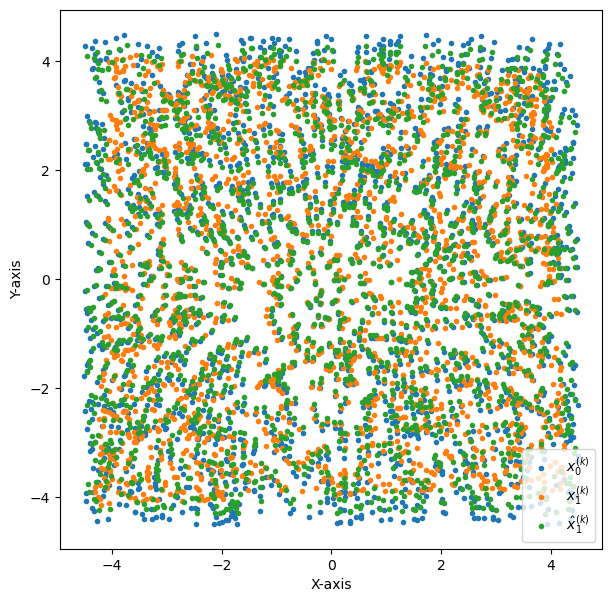
\includegraphics[width=0.65\textwidth]{images/nonlinear_vector_fields2.png}
\caption{scatter points}
\label{fig:3.2}
\end{figure}




\paragraph{Part 3.2: Approximate the vector field using radial basis functions}
Now, our objective is to approximate the vector field using radial basis functions (RBFs). The task involves determining an optimal number of centers, ranging between 100 and 1000, for the RBFs. The goal is to achieve an approximation such that 

\[
\frac{d}{ds} \psi(s, x(t)) \bigg|_{s=0} \approx \hat{f}_{\text{rbf}}(x(t)) = C\phi(x(t)).
\]

This approximation aims to capture the underlying dynamics of the process more effectively than linear methods, leveraging the flexibility and adaptability of RBFs.

In this task, we not only attempted the library function \texttt{scipy.interpolate.RBFInterpolator} to approximate the vector field but also used our own implementation, \texttt{rbf\_lstsq}. Their performances are nearly identical. The centers for the radial basis functions are randomly selected from the original data points. The labels of these center points correspond to the vectors\ref{vec} representing the changes in position.

When using different values of \(\epsilon\) and varying numbers of center points \(L\), the estimated vector field exhibits variations. To ensure that the approximate endpoints \(\hat{x}_1\) are relatively close to the known endpoints \(x_1\), i.e., to find a smaller value of \(\text{MSE}(\hat{x}_1, x_1)\), we will employ a grid search method to explore values for \(\epsilon\) and \(L\).

We utilized a heuristic approach to roughly determine the value of \(\epsilon\). \(\epsilon\) was computed as the average distance between all pairs of center points, yielding an approximate value of 5. Consequently, we fixed \(\epsilon\) at 5 and varied \(L\) from 100 to 1000 with a step size of 100 to obtain the corresponding Mean Squared Error (MSE). The results can be observed in Table \ref{table:results}.

\begin{table}[htbp]
  \centering
  \begin{tabular}{|c|c|}
    \hline
    \(L\) & \text{MSE} \\
    \hline
    100 & 0.005498255110276839 \\
    200 & 0.0004429862947538187 \\
    300 & 0.00034369626425355187 \\
    400 & 6.21790385068608e-05 \\
    500 & 1.3091339099161506e-05 \\
    600 & 2.3758776666557353e-06 \\
    700 & 3.2635934980513923e-06 \\
    800 & 1.7102134548916818e-05 \\
    900 & 2.342844970228924e-06 \\
    1000 & 5.269156875542863e-07 \\
    \hline
  \end{tabular}
  \caption{MSE for different values of \(L\) with \(\epsilon = 5\)}
  \label{table:results}
\end{table}

From the table, it can be observed that as \(L\) gradually increases, the obtained MSE decreases. Therefore, within the available range, \(L\) of 1000 is the most favorable choice. 

Next, we fix \(L\) at 1000 and further explore the values of \(\epsilon\). Using the same method, we conducted a search for 
\( \epsilon \) in the range of 0.01 to 200. We observed that the MSE achieves smaller values within the interval of 
\( \epsilon \) from 0.2 to 0.5. Since the selection of center points is random, the optimal \( \epsilon \) may vary. However, within this range, the choice of \( \epsilon \) has a minimal impact on the approximation results. Therefore, we choose to set \( \epsilon \) to 0.25.

When \(L\) is 1000 and \(\epsilon\) is 0.25, the resulting MSE is \(7 \times 10^{-12}\). This is significantly smaller compared to the MSE obtained using a linear operator to estimate the vector field. The estimated \(\hat{x}_1\) is plotted together with the original \(x_0\) and \(x_1\) in Figure \ref{fig:3.3}. It can be observed from the graph that all \(x_1\) points are covered by \(\hat{x}_1\). This indicates a quite satisfactory result for the approximation.


\begin{figure}[H]
\centering
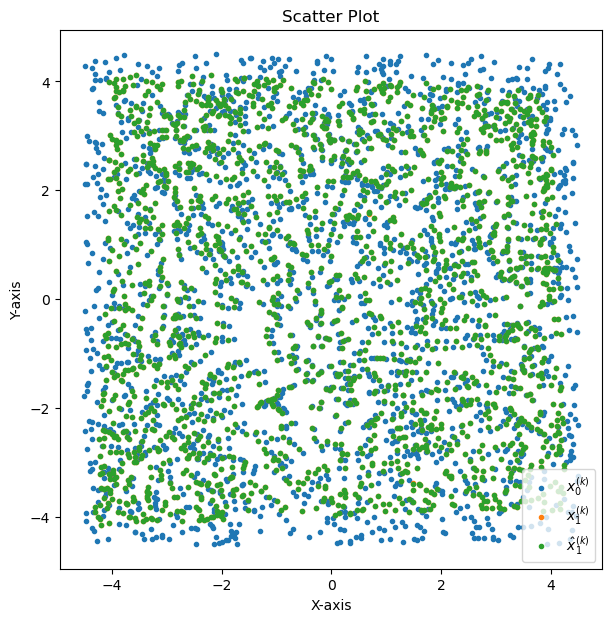
\includegraphics[width=0.65\textwidth]{images/nonlinear_vector_fields3.png}
\caption{scatter points}
\label{fig:3.3}
\end{figure}


In addressing the question of whether the vector field is linear or nonlinear, although there are multiple approaches to make such a determination, this question closely follows the analysis of MSE. Therefore, we will assess whether the vector field is linear or nonlinear from the perspective of MSE.

The results suggest that the vector field is more likely to be nonlinear. The RBF (Radial Basis Function) approximation significantly outperformed the linear approximation, indicating that a linear model is less likely to accurately capture the underlying behavior of the vector field. The superior performance of the RBF approximation implies a higher likelihood of nonlinear relationships within the vector field.

\paragraph{Part 3.3: states of the system}
After approximating the vector field using radial basis functions (RBF), we can visualize the vector field using the obtained RBF. The specific process is as follows: for the x-coordinate, 50 uniformly distributed points are generated within the range of -4.5 to 4.5; similarly, for the y-coordinate, another set of 50 uniformly distributed points is generated within the same range. In this way, a 2D grid containing 50x50 points is created, evenly distributed within the specified range. These points are then fed into the RBF, resulting in a series of vectors. By plotting these vectors on a 2D graph, we obtain a visualization of the vector field. The visualization is depicted in Figure \ref{fig:3.4}.

\begin{figure}[H]
\centering
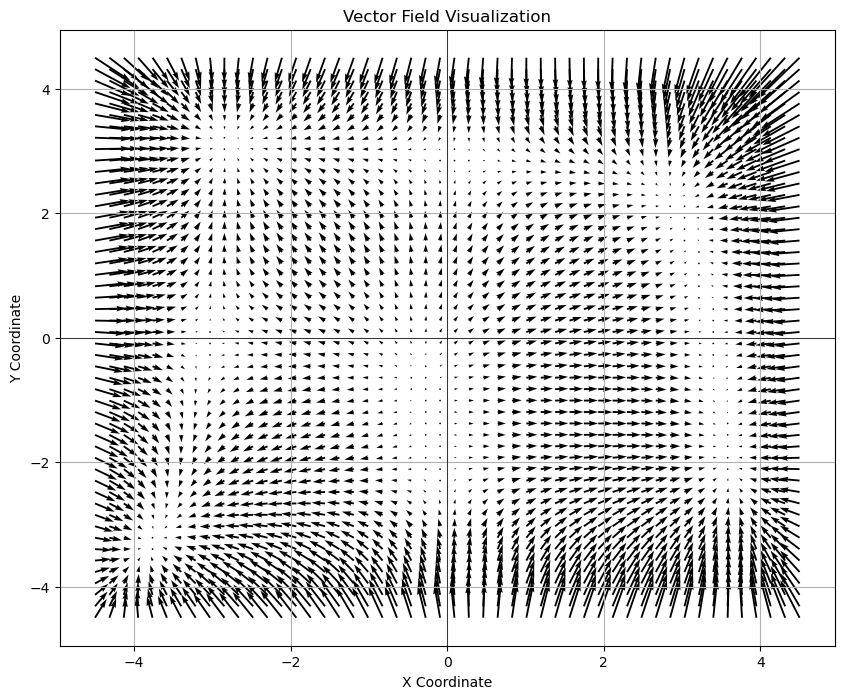
\includegraphics[width=0.65\textwidth]{images/nonlinear_vector_fields4.png}
\caption{vector field}
\label{fig:3.4}
\end{figure}

The steady states of a nonlinear vector field are the points where the vector field becomes zero, indicating that there is no change in the system at those points.

Seeking numerical solutions where the radial basis function (RBF) evaluates to zero can be challenging. However, we can pursue an analytical solution. We generated 1000 uniformly distributed points for both the x and y coordinates within the range of -4.5 to 4.5. This results in a 2D grid containing 1000x1000 points. Subsequently, these points are input into the RBF, and when the resulting function values approach zero vector, we consider these points as steady states. We set the threshold to \(8 \times 10^{-4}\), indicating that a vector is considered a zero vector when both its x and y components are below this threshold simultaneously. To better visualize the obtained points, we plotted them on the previous image, resulting in Figure \ref{fig:3.5}.

\begin{figure}[H]
\centering
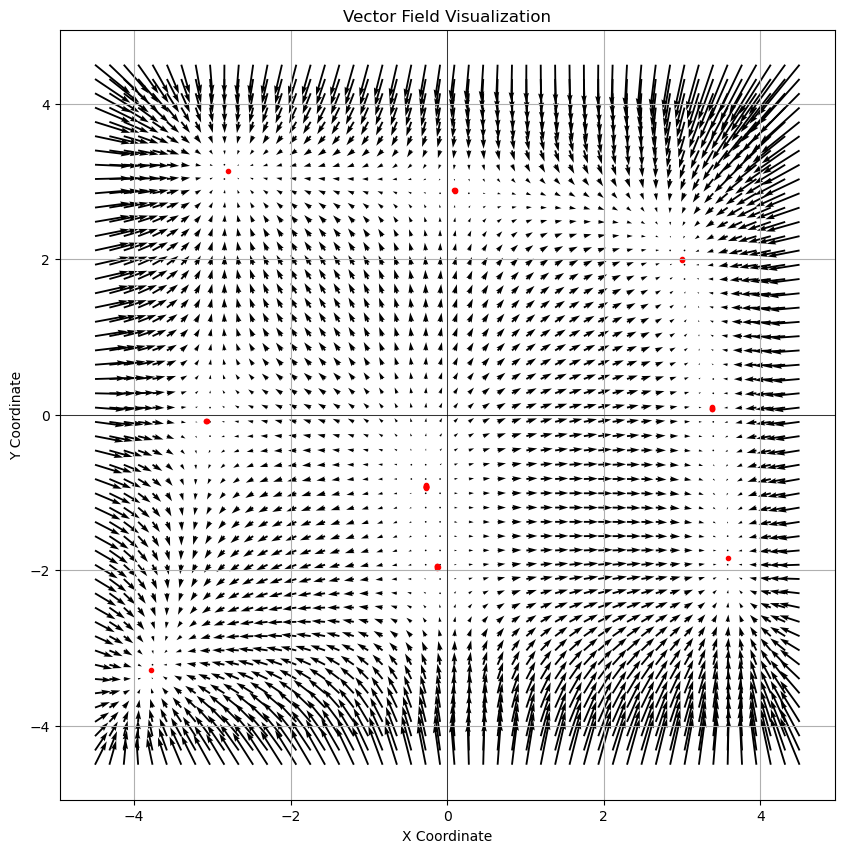
\includegraphics[width=0.65\textwidth]{images/nonlinear_vector_fields5.png}
\caption{vector field}
\label{fig:3.5}
\end{figure}

From the figure, we intuitively observe that the dynamical system has 9 steady states. In fact, among 1,000,000 input points, 28 meet the specified conditions. Some of them are quite close to each other, so it appears as if there are only 9 points. To obtain the states, we first retain one significant digit for the numerical values of these 28 points. Then, we eliminate the duplicates. Finally, we get 9 steady states are as follows: 

\begin{align*}
(-3.1, -0.1), (-2.8, 3.1), (-0.3, -0.9), (-0.1, -2.0), (-3.8, -3.3), (0.1, 2.9), (3.0, 2.0), (3.4, 0.1), (3.6, -1.8)
\end{align*}

In the previous exercise, we discussed the phase portraits exhibited by the linear system under different \(A\). However, this system, with 9 steady states, is completely distinct from any previous linear ones. Additionally, assuming that this system is represented accurately by the obtained radial basis function (RBF), it can be expressed as \(\hat{f}_{\text{rbf}}(x(t)) = C\phi(x(t))\). Due to the introduction of the nonlinearity in the function \(\phi(\cdot)\), \(C\phi(x(t))\) cannot be obtained from \(Ax(t)\) through a linear transformation. However, \(\hat{f}_{\text{linear}}(x(t)) = Ax(t)\) represents a linear system. Thus, it can be concluded that this system cannot be topologically equivalent to a linear system.


\end{task}